Consider the wave equation posed on the infinite domain $x\in(-\infty,\infty)$:
          $$ u_{tt}(x,t) = u_{xx}(x,t),
               \qquad -\infty < x < \infty,
               \quad   t>0 \eqno{(*)}$$
    with initial conditions $u(x,0) = \psi(x)$ and $u_t(x,0) = \gamma(x)$.

\def\xt{\widetilde{x}}
\def\ttil{\widetilde{t}}
     At a given point $(\xt,\ttil@@)$, 
      with $\xt\in(-\infty,\infty)$ and $\ttil>0$, 
      the solution $u(\xt,\ttil)$ of the wave equation
      is only affected by some portion of the initial data.  
      In other words, $u(\xt,\ttil)$ is only
      influenced by $\psi(x)$ and $\gamma(x)$ for $x\in[a,b]$, where 
      $a$ and $b$ will depend upon $\xt$ and $\ttil$.
      This interval $[a,b]$ is called the \emph{domain of dependence}
      of the solution at $(\xt,\ttil@@)$.

\begin{enumerate}
\item[(a)]
      Determine the domain of dependence of the solution to the wave
      equation~$(*)$ at $(\xt,\ttil@@) = (0,1)$.
\end{enumerate}

      Now consider the heat equation on an unbounded domain:
       \[ u_{t}(x,t) =  u_{xx}(x,t), \qquad  -\infty < x < \infty\]
      with initial data
       \[ u(x,0) = \psi(x).\]
      Like d'Alembert's solution, there exists a formula for the
      solution of the heat equation on this domain:
      for all $t>0$,
       \[ u(x,t) = {1\over 2\sqrt{\pi t}} 
                  \int_{-\infty}^\infty e^{-(s-x)^2\over 4t} \psi(s)\, \dop s.\]
     
\begin{enumerate}
\item[(b)] What is the domain of dependence of this solution to the
      heat equation at $(\xt,\ttil@@)=(0,1)$\,?\\
      Contrast the physical implications of the domains of dependence
      for the heat and wave equations.

\vspace*{1em}
\item[(c)] Consider the \emph{wave} equation with discontinuous 
      initial data
     \[ \psi(x) = \left\{\begin{array}{ll} 0, & x < 0; \cr 1, & x\ge 0;
                   \end{array}\right. \qquad
        \gamma(x) = 0.\]
      On one plot, superimpose solutions to this equation at the four times $t=0, 1/2, 1, 2$.\\
      (Notice how the discontinuity in the initial data is propagated in time.)

\vspace*{1em}
\item[(d)] Now consider the \emph{heat} equation with the same starting data
     \[ \psi(x) = \left\{\begin{array}{ll} 0, & x < 0; \cr 1, & x\ge 0.
                   \end{array}\right.\]
      Using the formula for $u(x,t)$ given above, produce solutions to this equation
      at the four times $t=0, 0.01, 0.1, 1$.  What happens to the discontinuity for $t>0$?

      \vspace*{1em}
      Important hint: You will need to compute some nasty integrals here that you
      cannot work out entirely by hand.  To produce your plots, use MATLAB's 
      \verb|erfc| command.  For example,
      \[  {2\over \sqrt{\pi}} \int_{\tt z}^\infty e^{-y^2} \, \dop y = {\tt erfc(z)}.\]
\end{enumerate}


%%%%%%%%%%%%%%%%%%%%%%%%%%%%%%%%%%%%%%%%%%%%%%%%%%%%%%%%%%%%%%%%%%%%%%%%%%%%%%%
\ifthenelse{\boolean{showsols}}{\begin{solution}
\begin{enumerate}
\item Recall that the general solution of the wave equation on an unbounded domain
      takes the form
     \[ u(x,t) = {\textstyle{1\over2}}\big(\psi(x-t) + \psi(x+t)\big) 
                   + {\textstyle{1\over2}}\int_{x-t}^{x+t} \gamma(s)\, ds.\]
      From this it follows that 
     \[ u(0,1) = {\textstyle{1\over2}}\big(\psi(-1) + \psi(1)\big) 
                   + {\textstyle{1\over2}}\int_{-1}^{1} \gamma(s)\, ds.\]
      Since the solution at $x=0$ and $t=1$ depends on $\gamma(s)$ for all
      $s\in[-1,1]$ and $\phi$ at $x=\pm 1 \in [-1,1$, we note that the 
      domain of dependence is the interval $[-1,1]$.

\item Since the solution to the heat equation in an unbounded domain depends
      on $\phi(s)$ for all values of $s\in(-\infty,\infty)$, the domain of 
      dependence at $x=0$ and $t=1$ consists of the entire real line, $(-\infty,\infty)$.

      {[Graders: please accept a variety of reasonable solutions to this problem.]}
      For the wave equation, the initial condition takes a finite time to propagate:
      for example, it takes one full time unit for the value of $\psi(\pm 1)$ to affect
      the solution $u$ at the point $x=0$.  In contrast, in the heat equation, with its
      domain of dependence of $(-\infty,\infty)$, the value of the initial condition at 
      any single point \emph{instantaneously} affects the solution at all other points.
      So, the initial distribution of heat instantly affects the heat at all other points.

\item Since $\gamma(x) = 0$ for all $x$, the solution to the wave equation is simply
     \[ u(x,t) = {\textstyle{1\over2}}\big(\psi(x-t) + \psi(x+t)\big) 
               = \left\{\begin{array}{ll}
                  0, &  x < -t; \\
                 1/2 &  -t \le x < t;\\
                  1, &  x > t. 
                 \end{array}\right. \]
       The requested plot of the solution is shown below; code follows at the end of the problem.
       \begin{center}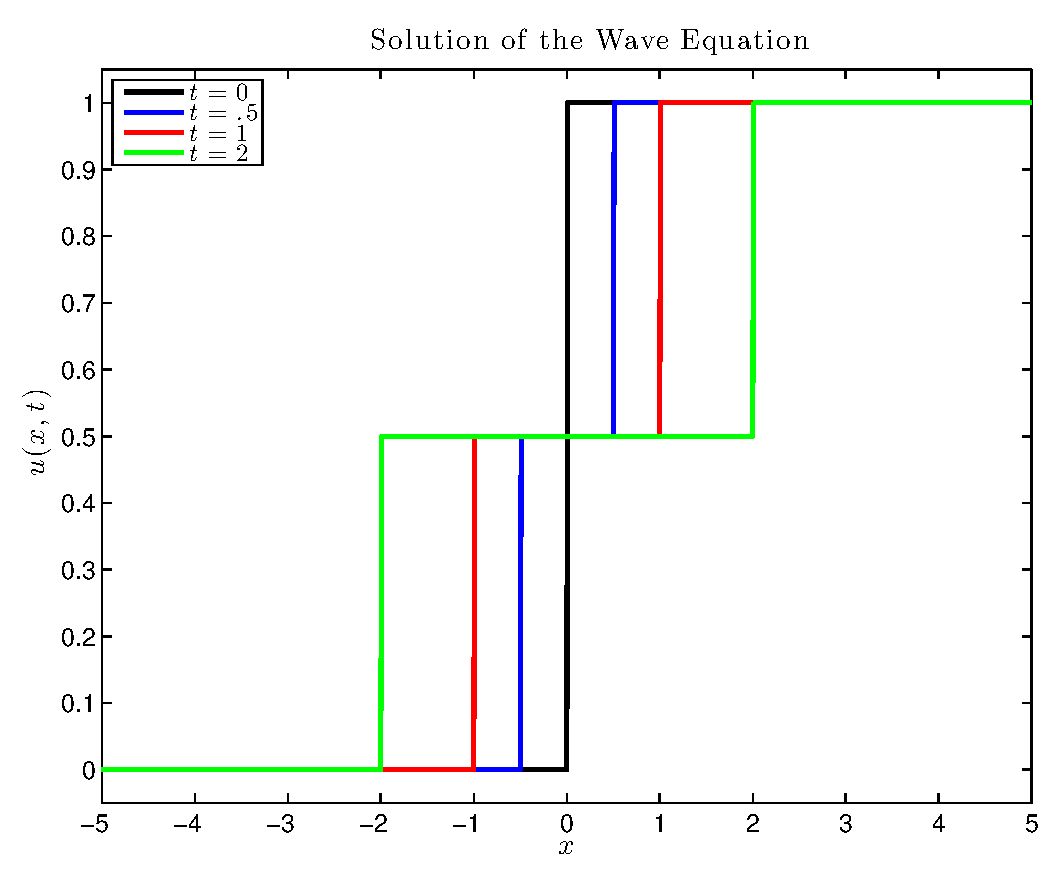
\includegraphics[scale=0.7]{heat_v_wave1}\end{center}

\item For the specified initial condition, the solution takes the form
       \[ u(x,t) = {1\over 2\sqrt{\pi t}} 
                  \int_{-\infty}^\infty e^{-(s-x)^2\over 4t} \psi(s)\, \dop s
                 = {1\over 2\sqrt{\pi t}} 
                  \int_{0}^\infty e^{-(s-x)^2\over 4t} \, \dop s.\]
      To compute the integral, use the substitution $y = (s-x)/(2\sqrt{t})$, so that
      $\dop y = 1/(2 \sqrt{t})\,\dop s$ to compute
       \[ \int_{0}^\infty e^{-(s-x)^2\over 4t} \, \dop s
          =2\sqrt{t} \int_{-x/(2\sqrt{t})}^\infty e^{-y^2} \, \dop y.\]
      Hence
       \[ u(x,t) = {1\over \sqrt{\pi}} \int_{-x/(2\sqrt{t})}^\infty e^{-y^2} \dop y
                 = {1\over 2} {\tt erfc}(-x/(2\sqrt{t})).\]
       The requested plot of the solution is shown below; code follows at the end of the problem.
       \begin{center}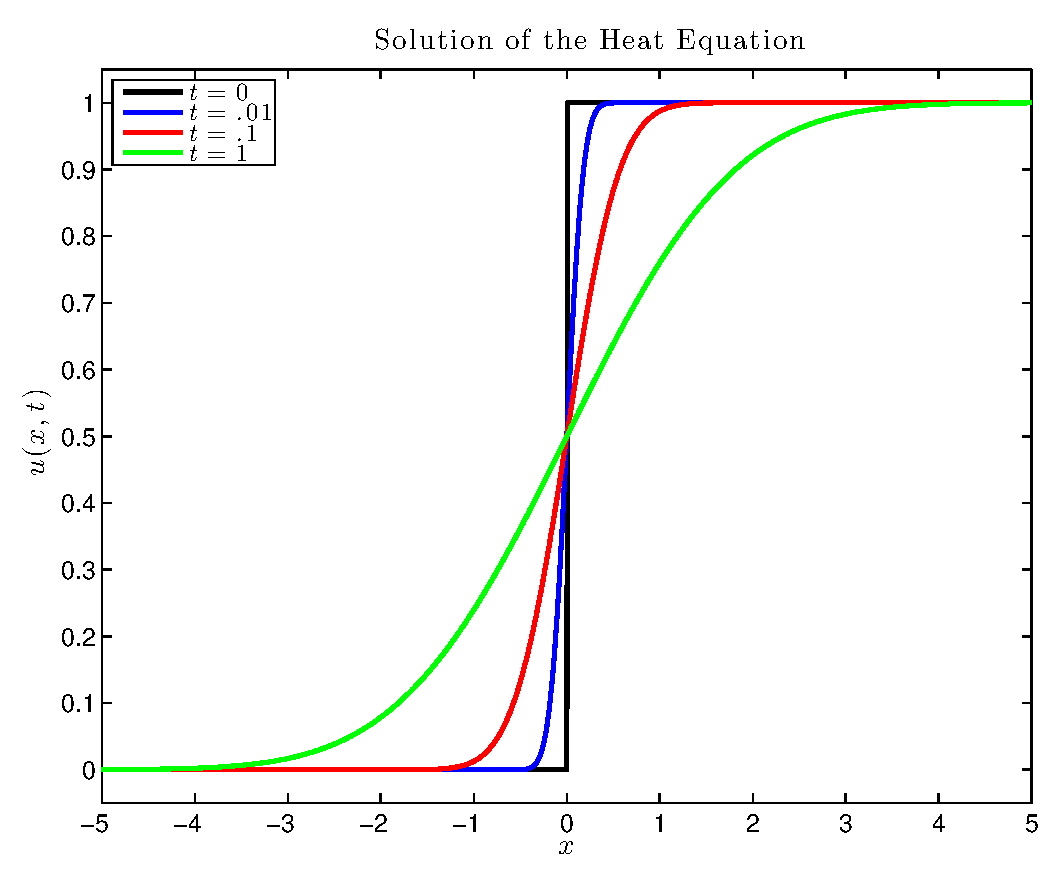
\includegraphics[scale=0.7]{heat_v_wave2}\end{center}
\end{enumerate}

\input heat_v_wave_code
\end{solution}}{}

